%
% Annual Cognitive Science Conference
% Sample LaTeX Paper -- Proceedings Format
%
% Original : Ashwin Ram (ashwin@cc.gatech.edu)       04/01/1994
% Modified : Johanna Moore (jmoore@cs.pitt.edu)      03/17/1995
% Modified : David Noelle (noelle@ucsd.edu)          03/15/1996
% Modified : Pat Langley (langley@cs.stanford.edu)   01/26/1997
% Latex2e corrections by Ramin Charles Nakisa        01/28/1997
% Modified : Tina Eliassi-Rad (eliassi@cs.wisc.edu)  01/31/1998
% Modified : Trisha Yannuzzi (trisha@ircs.upenn.edu) 12/28/1999 (in process)
% Modified : Mary Ellen Foster (M.E.Foster@ed.ac.uk) 12/11/2000
% Modified : Ken Forbus                              01/23/2004
% Modified : Eli M. Silk (esilk@pitt.edu)            05/24/2005
% Modified : Niels Taatgen (taatgen@cmu.edu)         10/24/2006
% Modified : David Noelle (dnoelle@ucmerced.edu)     11/19/2014

%% Change ''letterpaper'' in the following line to ''a4paper'' if you must.

\documentclass[10pt,letterpaper]{article}

\usepackage{cogsci}
\usepackage{pslatex}
\usepackage{apacite}
\usepackage{amsmath,amssymb}
\usepackage{graphicx}
\usepackage{subcaption}
\usepackage{color}
\usepackage{url}
\usepackage{todonotes}
\usepackage{mathtools}
\usepackage{stmaryrd}
\usepackage{booktabs}
\usepackage{array}
\graphicspath{{./figures/}}

%\newcommand{\url}[1]{$#1$}

\definecolor{Red}{RGB}{178,34,34}
\newcommand{\red}[1]{\textcolor{Red}{#1}}
\newcommand{\rdh}[1]{\textcolor{Red}{rdh: #1}}
\definecolor{Green}{RGB}{10,200,100}

 \newcommand{\denote}[1]{\mbox{ $[\![ #1 ]\!]$}}


\newcommand{\subsubsubsection}[1]{{\em #1}}
\newcommand{\eref}[1]{(\ref{#1})}
\newcommand{\tableref}[1]{Table \ref{#1}}
\newcommand{\figref}[1]{Fig.~\ref{#1}}
\newcommand{\appref}[1]{Appendix \ref{#1}}
\newcommand{\sectionref}[1]{Section \ref{#1}}

\title{Graphical convention formation during visual communication}

% \author{\begin{tabular}[htbp]{c@{\extracolsep{1em}}c@{\extracolsep{1em}}c@{\extracolsep{1em}}c} \\
% {\large \bf Megumi Sano} & {\large \bf Robert X. D. Hawkins} & {\large \bf Noah D. Goodman} & {\large \bf Judith E. Fan}\\
% Department of Psychology & Department of Psychology & Department of Psychology & Department of Psychology \\
% Stanford University & Stanford University & Stanford University & UC San Diego \\
% \texttt{megsano@stanford.edu} & \texttt{rxdh@stanford.edu} & \texttt{ngoodman@stanford.edu} & \texttt{jefan@ucsd.edu} \\
% \end{tabular}
% }

\author{\large \bf Anonymous Authors}

\begin{document}
\maketitle

\begin{abstract}
Humans have developed sophisticated graphical conventions to communicate, ranging from maps to musical notation to modern data visualization. 
How do these abstract visualizations derive meaning? 
A key hypothesis is that their capacity to be effective carriers of meaning is driven by the functional needs of the people who develop and use them to communicate. 
Here we investigated the formation of novel graphical conventions across extended visual communication between two people. 
We developed a drawing-based reference game in which two participants repeatedly communicate about visual objects. 
On each trial, both players were shown an array of four objects; the sketcher’s goal was to draw one of these, the target, so that the viewer could guess the target as quickly as possible. 
The game included two sets of objects: objects in one set were drawn repeatedly, while those in a control set were drawn once at the beginning and again at the end of the game. 
Across repetitions, we find that pairs discover increasingly sparse, yet effective and internally consistent ways of depicting them. 
While we observe gains in communication efficiency for all objects, they were greater for the repeated objects, suggesting both task-level and object-level benefits of repeated communication. 
Moreover, different pairs discovered different solutions for efficient communication, revealing the existence of multiple equilibria in the space of graphical conventions. 
Taken together, our findings suggest that repeated visual communication promotes the emergence of depictions whose meanings are increasingly determined by social context rather than their perceptual properties alone.

\textbf{Keywords:}
sketch understanding; drawing; iconicity; visual abstraction; social coordination

\end{abstract}

\section{Introduction}

\red{Seeding intro section with text from abstract ...}

\red{Big picture: What do we mean by graphical conventions? Why are they cool and important to study?}
Over time, humans have developed sophisticated systems to communicate complex ideas in compact graphical form, ranging from maps to musical notation to modern data visualization. 
How do these abstract visualizations derive meaning? 
A key hypothesis is that their capacity to be effective carriers of meaning is driven by the functional needs of the people who develop and use them to communicate. 


As a consequence, the way these 

 may come to denote objects through culturally-specific conventions much the same way that verbal labels denote objects \cite{goodman1976languages,gombrich1969art}. 
While a strong version of this view is controversial \cite{kennedy1975drawings,Gibson:1971fj,abell2009canny}, the interpretation of drawings \textit{can} crucially depend on social and cultural factors. 
Indeed, many drawings that people use to communicate are quite sparse, emphasizing information that is currently relevant, and omitting other details. 
In the appropriate context, even a few strokes can express the identity of a face \cite{bergmann2013impact}, a suggested route \cite{agrawala2001rendering}, or an intention to act \cite{Galantucci:2005uh}. 
Over time, repeated communication between members of the same community can lead to novel graphical conventions \cite{Garrod:2007wk,fay2010interactive}. 
However, in the absence of contextual cues or prior interaction history, such sparse representations may be insufficient to communicate specific meanings \cite{Healey:2007vq}.

\red{What prior work has been done to understand them?}


\red{perimetric complexity to quantify changes to drawings across repetitions, some exploration of role of viewer feedback, some initial use of recognition task to probe properties of drawings in absence of interaction history}
\cite{garrod_foundations_2007}

\red{some compositionality using pictionary task}
\cite{theisen2010systematicity}

\red{abstraction, systematicity using pictionary task}
\cite{healey2007graphical}

\red{exploration of lexical coordination in linguistic reference}
\cite{ClarkWilkesGibbs86_ReferringCollaborative}
\cite{HawkinsFrankGoodman17_ConventionFormation}

\red{What is the gap in knowledge that this paper aims to help fill?}

\red{What is the approach we take to fill that gap?}
Here we investigated how novel graphical conventions form across extended visual communication between agents. 
Specifically, we used an online drawing-based reference game in which two players repeatedly communicate about visual objects. 
On each trial, both players were shown an array of four objects; the sketcher’s goal was to draw one of these, the target, so that the viewer could guess the target as quickly as possible. 
The game included two sets of objects: objects in one set were drawn repeatedly, while those in a control set were drawn once at the beginning and again at the end of the game. 

\red{High-level summary of main findings and contributions}

We make the following main contributions:
-- tighter control over stimulus set and communicative demands
-- deeper experimental exploration of the degree to which changes in communication performance reflect interaction history vs. either production task practice (sketcher getting better at producing sketches overall) or comprehension task practice (viewer getting better at matching sketches overall)
-- using task setup that is in principle image-computable
-- novel use of modern vision models to characterize high-level perceptual information in sketches

Across repetitions, we find that pairs discover increasingly sparse, yet effective and internally consistent ways of depicting them. 
While we observe gains in communication efficiency for all objects, they were greater for the repeated objects, suggesting both task-level and object-level benefits of repeated communication. 
Moreover, different pairs discovered different solutions for efficient communication, revealing the existence of multiple equilibria in the space of graphical conventions. 
Taken together, our findings suggest that repeated visual communication promotes the emergence of depictions whose meanings are increasingly determined by social context rather than their perceptual properties alone.

\section{Part I: How does repeated reference support successful visual communication?}

%% intro to this section
\rdh{eventually need to compress these methods quite a bit (participants can be 1 sentence, much less detail about stim selection and procedure, etc.)} 

To investigate the formation of \textit{ad hoc} graphical conventions in a naturalistic setting, we developed a visual communication task in which people repeatedly referred to familiar real-world objects, but where pre-existing graphical conventions were unlikely to be sufficient to succeed. 
In line with prior studies of repeated verbal communication \cite<e.g>{ClarkWilkesGibbs86_ReferringCollaborative} and visual communication about verbal stimuli \shortcite<e.g.>{garrod_foundations_2007}, we hypothesized that repeated visual reference to a visual object would lead to more efficient communication about that object.
Departing from prior studies, our experiment critically includes a control set of visual objects that are not repeatedly referenced, which allows us to measure the extent to which changes in efficiency are item-specific or attributable to task practice. 

%% methods
\subsection{Methods: Visual Communication Experiment}

\subsubsection{Participants} A total of 138 unique participants (verify), who were recruited via Amazon Mechanical Turk (AMT) and grouped into pairs, completed the experiment.
They were provided a base compensation of \$1.50 for participation and earned up to \$0.04 bonus for each correct trial, inversely proportional to the amount of time taken. 
\red{what was exclusion criteria? -- definition of crazy in df generation helpers?}
Data from two pairs were excluded due to unusually low performance on the task (i.e., proportion correct $<$3 s.d. below the mean).
In this and subsequent behavioral experiments, participants provided informed consent in accordance with the Stanford IRB.\footnote{All materials and data are available at \url{https://github.com/cogtoolslab/graphical_conventions}.}

\subsubsection{Stimuli} 
%% provide justification for why we're using sets of similar objects
%% provide justification for why we're using images of real-world objects

Our approach was to define sets of perceptually similar real-world objects belonging to the same basic-level category \cite{MervisRosch81_CategorizationReview}.
To accomplish this, we utilize the collection of chair objects in the ShapeNet database \cite{chang2015shapenet}.
This collection contains objects that are geometrically complex, highly diverse, and abundant in the real world.
To identify groups of perceptually similar chairs within the collection, we first extracted high-level visual features of each of the 3,096 object images using a pre-trained deep convolutional neural network, VGG-19 \cite{simonyan2014very}. 
We then applied principal component analysis and $k$-means clustering to the model's top-layer feature representation of the images. 
This yielded 70 clusters containing between 2 and 80 objects each (\red{verify}).
Based on the results of this feature extraction and clustering procedure, we defined two categories of perceptually similar objects containing eight exemplars each (Fig.~\ref{fig:1a}). 

% In order to identify groups of objects that are drawn similarly prior to training, we applied a clustering algorithm (affinity propagation with damping = 0.9; \cite{frey2007clustering}) to the model's top-layer feature representation of drawings from the same dataset analyzed above \cite{Eitz:2012dk}. This yielded 16 clusters containing between 3 and 20 objects each. Among clusters containing at least 8 objects, we defined 8 ``visual categories'' containing 8 objects each (Table \ref{cluster_obj_list}). Each participant was randomly assigned two of these categories, and only the 16 objects from these two categories appeared as drawing targets during their session.

%% Shapenet
%% Describe goal (groups of highly similar objects that would be hard to distinguish)


%% Figure 1 around here: (A) Stimuli. (B) Task (Sketcher/Viewer interface)
\begin{figure}
\begin{subfigure}{0.23\textwidth}

\includegraphics[width=\linewidth]{figures/fig_a.png}
\caption{Stimuli} \label{fig:1a}
\end{subfigure}
\hspace*{\fill}
\begin{subfigure}{0.23\textwidth}

\includegraphics[width=\linewidth]{figures/fig_b.png}
\caption{Sketcher / Viewer interface} \label{fig:1b}
\end{subfigure}
\caption{} \label{fig:1b}
\end{figure}

\subsubsection{Procedure} 

%% Trial-level event structure

Drawings were collected in the context of an online, sketching-based reference game using the framework described in \citeA{Hawkins15_RealTimeWebExperiments}. 
The game involved two players: a \textit{sketcher} who aims to help a \textit{viewer} pick out a target object from a set of distractor objects by representing it in a sketch. 
On each trial, both participants were shown the same array of four objects; however, the positions of these objects were randomized for each participant. 
One of the four objects was highlighted on the sketcher's screen to designate it as the target.

%% Trial-level objective of sketcher and viewer
Sketchers drew using black ink on digital canvas (pen width = 5 pixels; 300 $\times$ 300 pixels) embedded in a web browser window. 
Participants drew using the mouse cursor, and were not able to delete previous strokes. Each stroke was rendered on the viewer's screen immediately upon the completion of each stroke. 
The sketcher was instructed to take no longer than 30 seconds to produce their drawings. 
The viewer was allowed guess the identity of the drawn object by clicking one of the four objects in the array even when the sketcher had not completed the drawing. 
Both participants received immediate task-related feedback: the sketcher learned when and which object the viewer had clicked, and the viewer learned the true identity of the target. 
Otherwise, the viewer had no other means of communicating with the sketcher. 
Both participants earned accuracy bonus points for each correct response. 
If the correct response was made under the 30-second time limit, they also received speed bonus points inversely proportional to the time taken until the response.

%% Two conditions: repeated and control

% Each pair of participants was randomly assigned two of these categories, and only the 16 objects from these two categories appeared as drawing targets during their session.

Each pair of participants was randomly assigned two sets of four objects: one set was was assigned to the repeated condition; the other to the control condition.
In order to explore the degree to which the effects of repeated communication were object-specific, we varied the perceptual similarity between the two sets across pairs. 
Specifically, in half of the pairs (N=XX pairs), one set contained four randomly sampled objects from one category and the second set contained the remaining four objects from the same category. 
In the other half of pairs (N=XX pairs), one set contained four randomly sampled objects from one category and the second set contained four randomly sampled objects from the other category.
The assignment of each set to the repeated and control conditions was randomized across pairs. 

The communication task consisted of three phases. 
During the \textit{repeated} phase, the sketcher drew the four repeated objects six times each, in an interleaved order.
Specifically, there were six repetition epochs wherein each object in the repeated set served as the target exactly once, and object order was randomized across repetition cycles. 
Before and after the \textit{repeated} phase, the sketcher drew all eight objects one time each, again in randomly interleaved order. 
Including the control condition in this pre-post design allowed us to assess the specificity of repetition effects: control objects from the same category were maximally perceptually similar to the repeated objects but were not repeatedly drawn, and control objects from the other object category provided a measure of the generic effects of production task practice. 

\subsection{Result: communication becomes more efficient across interaction}

\begin{figure}
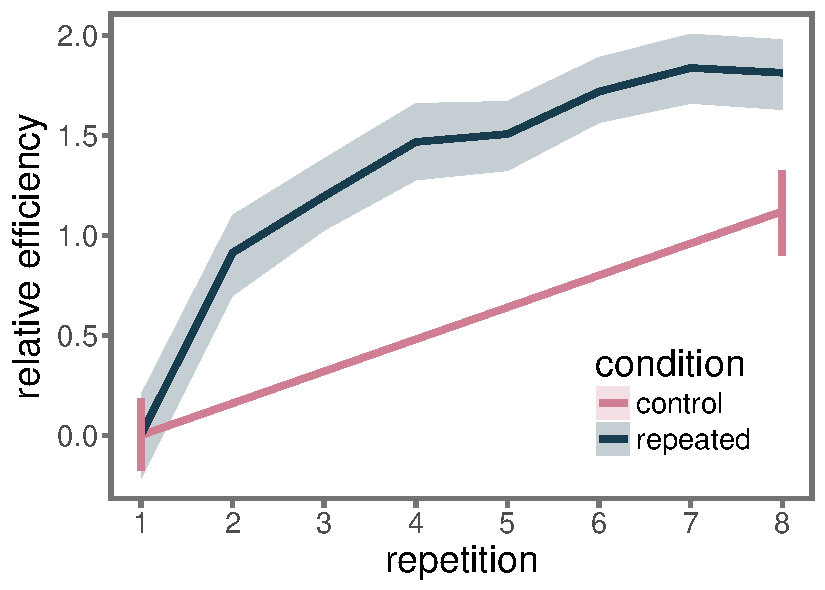
\includegraphics[width=\linewidth]{figures/refgame_BIS_timeseries.pdf}
\caption{Communication efficiency for repeated and control objects across repetitions. Efficiency was computed using a metric that combines both speed and accuracy, and is plotted relative to performance on the first repetition.} \label{refgame_bis}
\end{figure}

We operationalized communicative efficiency using a composite behavioral measure that accounts for both accuracy (proportion of successful listener responses) and speed (the time elapsed during drawing).
More specifically, we normalize both accuracy and drawing duration within each game and take the difference between these scores \cite<the \emph{balanced integration score,}>{Liesefeld2018}.
To compare the effect of repetition across the control and repeated conditions, we conducted a mixed-effects regression including a maximum random effect structure with random intercepts, slopes, and interactions for each pair of participants and each target object. 
While pairs became increasingly efficient between the pre-test and post-test for both control and repeated objects, we also found a significant interaction: sketches of repeated targets showed a greater increase in efficiency than the control targets which were shown only at the beginning and end ($b = X.XX. t = X.XX, p = X.XX$; see Figure \ref{refgame_bis}). 
%This ensures that the reduction in the drawing duration and number of strokes over time is not due to the players losing interest or becoming less motivated during the game. 
We find a similar effect when we examine number of strokes per sketch as the `speed' measure instead of drawing duration. 
Thus, \rdh{need short summary sentence}
%We clearly see that while the cost of sketching decreases, the accuracy of the viewer's guess of which object the sketch is referring to increases, suggesting that this reduction is meaningful.

%Successful communication was primarily quantified as the viewer's accuracy in identifying the target. 
%The investment of time was measured as the length of time between the beginning of the first stroke to the completion of the final stroke in each sketch, and the investment of ink was measured in two ways: as the number of strokes used for each sketch and the proportion of the drawing canvas filled by ink.

\section{Part II: What explains gains in communication efficiency?}

\subsection{Methods: Recognition Experiment}

%% need a better transition here (rather than `we were also interested'...)
While the repeated and control conditions in the drawing task help us investigate the importance of repeated communication in graphical convention formation, we are also interested in the effect of interaction-specificity on efficient communication. 

How does efficiency of graphical communication, measured by how accurately and quickly the viewer can select the target intended by the sketcher, change when we change the degree of interaction specificity? 
Here, we define interaction specificity based on both temporal structure (path dependence) and partner specificity. 
Therefore, we design several experiments that measure the recognizability of drawings and reaction times produced in the drawing task by third-party observers. 
The first is a yoked control design where each subject sees the sketches of all trials in one reference game with preserved temporal structure. 
In the second design, we manipulate partner specificity scrambling sketches within a repetition across reference games, so that each subject sees sketches from 40 trials, every four from four different reference games but with preserved temporal structure. In the last design,

% More about method design:
% Yoked
Just as in the communication task, a subject was given the role of a Viewer, with access to the same four-object context the original Sketcher in the reference game had access to and asked to select which object the drawing is referring to on each trial. 
The only difference between this design and the reference game is the absence of feedback -- because this is not a real-time two-player game, the Sketcher does not know which object the third-party viewer had guessed on each trial. 
The subject is awarded with a bonus system similar to the one in the reference game.

\subsection{Results: Gains in efficiency are not explained by task practice alone}


% With increasing repetition number, we saw a decrease in the average number of seconds taken from the start of the first stroke to the end of the last stroke of a sketch and in the average number of strokes required to draw it. Along with this cost reduction, we saw an increase in task performance, measured by the proportion of trials for which the viewer guesses the target accurately.


\begin{figure}
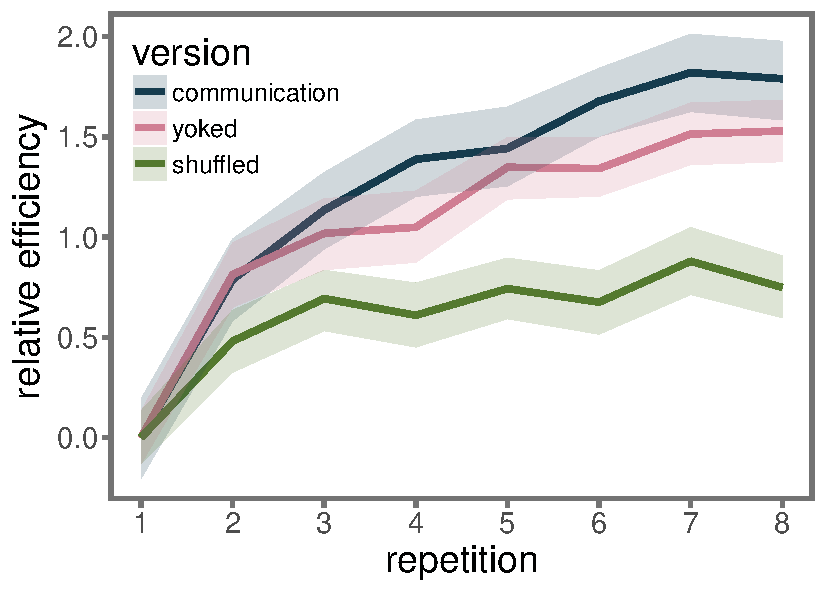
\includegraphics[width=\linewidth]{figures/recog_BIS_timeseries.pdf}
\caption{XX} \label{recog_bis}
\end{figure}

\section{Part III: How do visual features of sketches change across repetitions?}

\subsubsection{Sketches become more consistent across repeated interaction}

\red{Report results from yoked and scrambled recognition controls}

\subsubsection{Different pairs develop different graphical conventions} 
To analyze how the content of the sketches change over time, we extracted the high-level perceptual features of the drawings using a pre-trained convolutional neural network. 
(Explain more why this is appropriate.) 
We define the similarity between two sketches by the correlation between their respective features.
% perhaps move this similarity explanation in the earlier subsubsection.


\subsection{Discussion}

XXXX

%\vspace{-.30cm}
\section{\bf Acknowledgments}
\small
MS was supported by the Center for the Study of Language and Information at Stanford University. RXDH was supported by the Stanford Graduate Fellowship and the National Science Foundation Graduate Research Fellowship (DGE-114747). NDG was supported by ONR grant N000141310341 and a Sloan Foundation fellowship.
%\vspace{-.20cm}
\bibliographystyle{apacite}

\setlength{\bibleftmargin}{.125in}
\setlength{\bibindent}{-\bibleftmargin}

\bibliography{references}


\end{document}
